\documentclass[a4paper,10pt]{article}
\usepackage[left=2cm,top=2cm,right=2cm,bottom=2cm]{geometry}
\usepackage[utf8]{inputenc}
\usepackage{amsthm}
\usepackage{graphicx}
\graphicspath{ {images/} }

\newcommand{\mN}{{\mathbb N}}
\newcommand{\mZ}{{\mathbb Z}}
\newcommand{\cZ}{{\mathcal Z}}
\newcommand{\fL}{{\mathfrak L}}
\newcommand{\dst}{\displaystyle}

%opening
\title{}
\author{}
\date{}

\begin{document}

\maketitle
Carlos Alberto Gallegos Tena \\\\
Examen grupos\\\\
Para encriptar el mensaje ORDER A  PIZZA. Vamos a separar las letras en 2 y poner una X al final para que nos quede un número par. Entonces tenemos OR DE RA PI ZZ AX. Si los tomamos como números (sin la Ñ) nos queda \\\\
O=14 , R=17, D=03, E=04, R=17, A=00, P=15, I=17, Z=25, X=23.\\\\
Usando RSA, tenemos la fórmula de encriptación E tal que E(B)=$B^e mod$ n donde B son nuestros números (letras) que queremos encriptar. Entonces, tomando e=5 y n=1459, usando modular exponencial con 5=$(101)_2$, tenemos que:\\\\
La tabla muestra cómo se calculó el módulo del exponencial correspondiente.\\\\
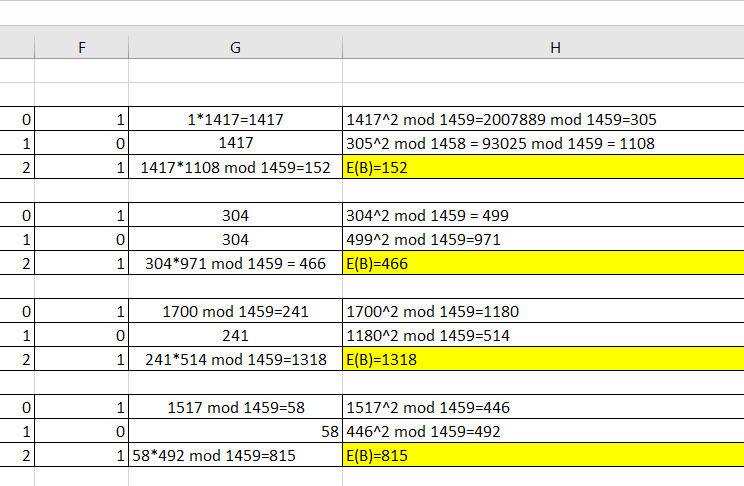
\includegraphics[scale=.8]{Captura de pantalla (53).png}\\\\
$1417^5 mod$  1459 = 0152\\\\
$0304^5 mod$  1459 = 0466\\\\
$1700^5 mod$  1459 = 1318\\\\
$1517^5 mod$  1459 = 0815\\\\
$2523^5 mod$  1459 = 0643\\\\

Por lo tanto, el cyphertext para ORDER A  PIZZA usando encriptación RSA con e=5 y n=1459 sería 0152 0466 1318 0815 0643.








\end{document}